\documentclass[10pt,letterpaper]{article}
\usepackage[letterpaper,margin=0.75in]{geometry}
\setlength\parindent{0pt}
\usepackage[sorting=none,backend=biber]{biblatex}
\usepackage{hyperref}
\usepackage{amsmath}
\usepackage{graphicx}
\begin{document} 

\textbf{Introduction: Heavy Loopers} \\

A charged heavy particle produced at the LHC may have a small transverse
momentum ($p_{\mathrm{T}}$), which makes it hard to travel through the inner
detector (ID) due to the bending caused by the magnetic field. The standard
ATLAS tracking algorithm usually requires a minimal amount of hits to
reconstruct a track, which means the particle has to pass a minimal number of
layers.  Therefore there exists a certain $p_{\mathrm{T}}$ threshold, for a
given charge, for the particle to be reconstructable hypothetically. This
becomes more critical when exotic multiple charged particles are considered as
the $p_{\mathrm{T}}$ threshold is lower as explained below. In this short note,
I performed some simple calculations to extract those thresholds. Such a
particle will spiral along the $z$-axis, leaving hits in the first few layers
of the ID with a clear pattern. We can name this signature as the ``Heavy
Loopers''. \\ 

\textbf{Obtain Track $p_{\mathrm{T}}$ via Radius, Charge and Magnetic Field}\\

Starting from simple approximation: 

\begin{equation}
\cdot\frac{v^{2}}{r} = m\cdot q \cdot B
\label{equ:1}
\end{equation}

One gets:

\begin{equation}
p_{\mathrm{T}} = q\cdot B \cdot r
\label{equ:2}
\end{equation}

Performing a simple dimensional analysis:

\begin{equation}
\begin{gathered}
[B] = [J][A^{-1}][L^{-2}],\\  
[r] = [L],\\
[q] = [e],\\
[qBr] = [J][A^{-1}][L^{-1}][e], \\  
[A] = [C][T^{-1}],\\
[J] = [C][V],\\
[qBr] = [V][T][e][L^{-1}] = 3e10\cdot[\frac{eV}{c}] = 0.3\cdot[\frac{GeV}{c}] \\
\label{equ:3}
\end{gathered}
\end{equation}

As a result, in ATLAS ($B = 2$ Tesla), a unit charge particle ($q = 1$), with a
track radius of one meter ($r = 1$ meter), has a $p_{\mathrm{T}}$ of 0.6 GeV.  \\

\textbf{Critical $p_{\mathrm{T}}$ for Loopers}

Let us assume that to make such a looper escape the tracking reconstruction, it
should not pass more than four tracking layers. The fourth pixel layer has a
radius of 122.5 mm. As a result, the critical track radius is therefore 61.25
mm. Using Equ.\ref{equ:3}, this gives a $p_{\mathrm{T}}$ of 0.036 GeV. Such low
$p_{\mathrm{T}}$ particles is only abundant if the production threshold is very
close to 13 TeV to have a very small $Q$. \\

However, in the context of multiple charged particles, this threshold vary. For
a particle with $q = 10$, this threshold reaches 0.36 GeV. If the critical
track radius is loosened to be the fifth layer of the ID, which is the first
layer of the SCT, corresponding to a radius of 299 mm, the threshold becomes ~
1 GeV. Figure~\ref{fig:qvsr} shows the $p_{\mathrm{T}}$ for a given
charge-radius combination.\\

\begin{figure}[!thb]
   \centering
   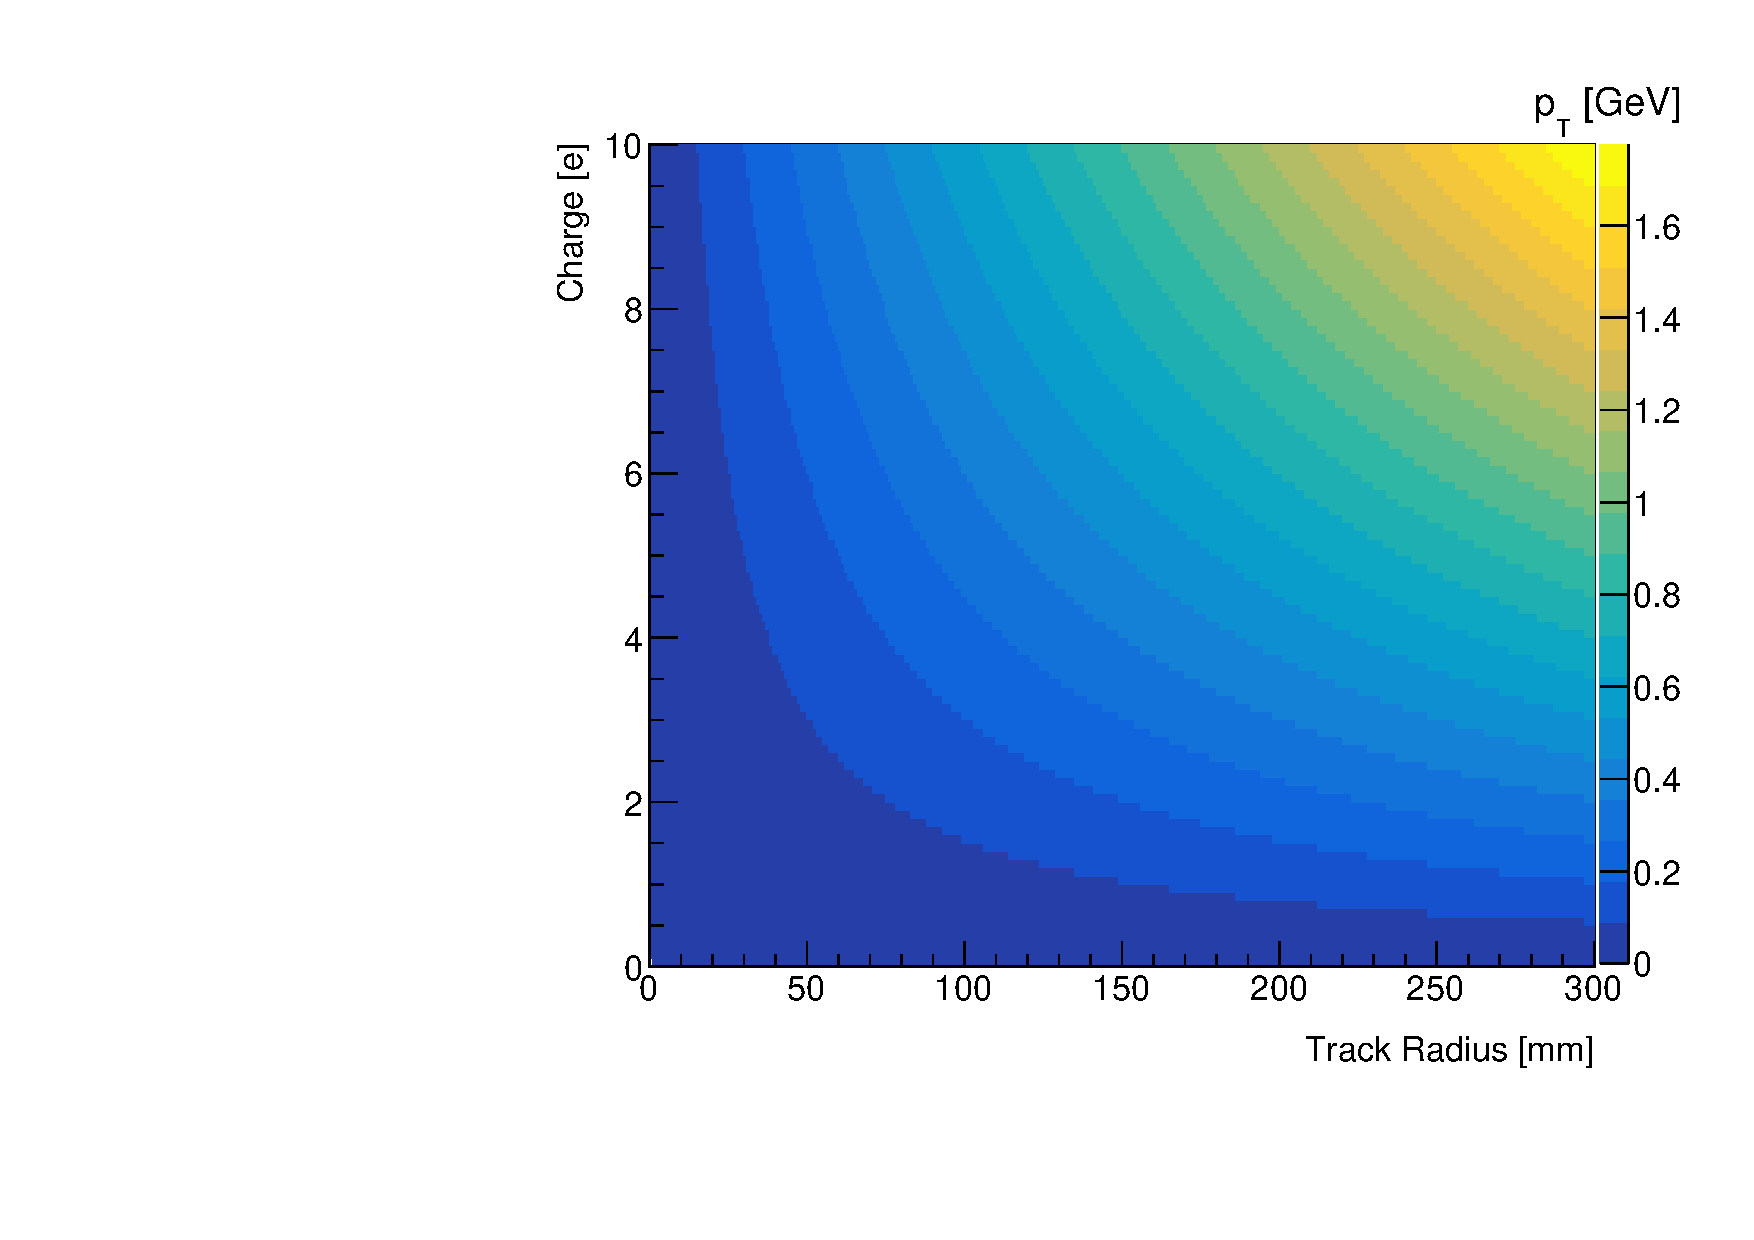
\includegraphics[scale=0.5]{qvsr.pdf}
   \caption{Distribution of $p_{\mathrm{T}}$ for a given charge ($y$-axis) and a given track radius ($x$-axis).}
   \label{fig:qvsr}
\end{figure}

\textbf{Experimental Signatures}

Particles with $p_{\mathrm{T}}$ below the threshold wil spiral along the
$z$-axis in the ID as illustrated in Figure~\ref{fig:looper}. Due to the
energy lost the separation in $z$ decreases in practice. However a strong
correlation still present between the hits left, forming a series of hits on
the same ID layer with nearly evenly separation in $z$ ($z$-line). For a
multiple charged particle, those hits are highly ionizing. If the particles are
not completely stable so that they decay after traveling for a certain distance
in $z$, this gives us a displaced vertex + $z$-lines. These are interesting
signatures that have not been considered so far.\\ 

\begin{figure}[!thb]
   \centering
   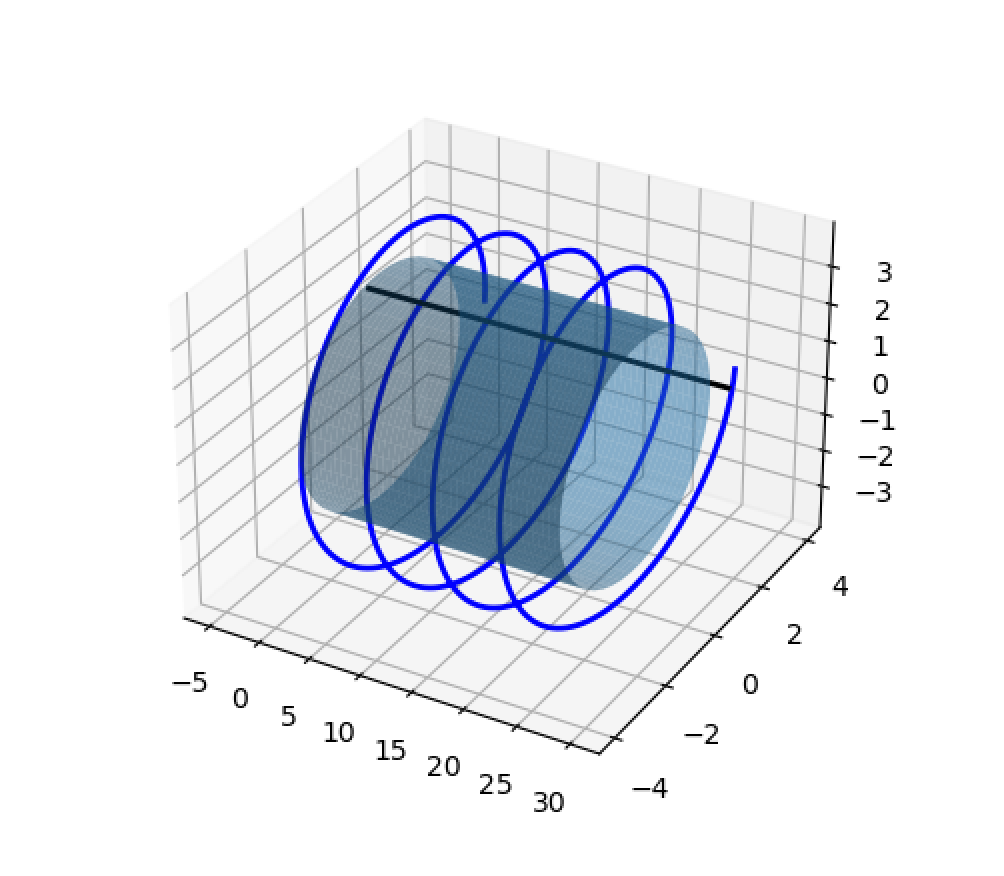
\includegraphics[scale=0.5]{spiralCartoon.png}
   \caption{Illustration of the ``Heavy Looper'' signature.}
   \label{fig:looper}
\end{figure}

\textbf{Discussion}

The ``Heavy Looper'' signature, or in general, the ``Looper'' signature, may
rise, for instance the soft pions produced in many BSM scenarios. In the
context of heavy stable multiple charged particle, when the particle has a very
large charge and extremely heavy (closing to the collision energy), the ``Heavy
Looper'' signature appears. In this note, I only considered the case where
standard track reconstruction is likely to fail, but in principle we do not
have to place this constraint. As long as the charged particle can re-enter the
ID volume, signatures similar to ``Heavy Looper'' still show up. To be
continued.

\end{document}
